\section{Conclusion}
By applying all these methods and combining them in a most profitable way, the Ferienakademie always ends up with nice results. These are usually presented in the final evening where the different courses come together and regard what the others did. But not only on the courses side, this summer school is a complete success. Motivated people from a lot of different fields come together for twelve days to work, study and -- most importantly-- have fun together. Ferienakademie succeeds at connecting these parts which sometimes get lost in regular studies and if you are willing to get involved you will get a lot out of it. A few more final expressions can be seen in \autoref{fig:durnholz} and \autoref{fig:Snow}.
\begin{figure}[ht]%
 	\begin{center}%
 		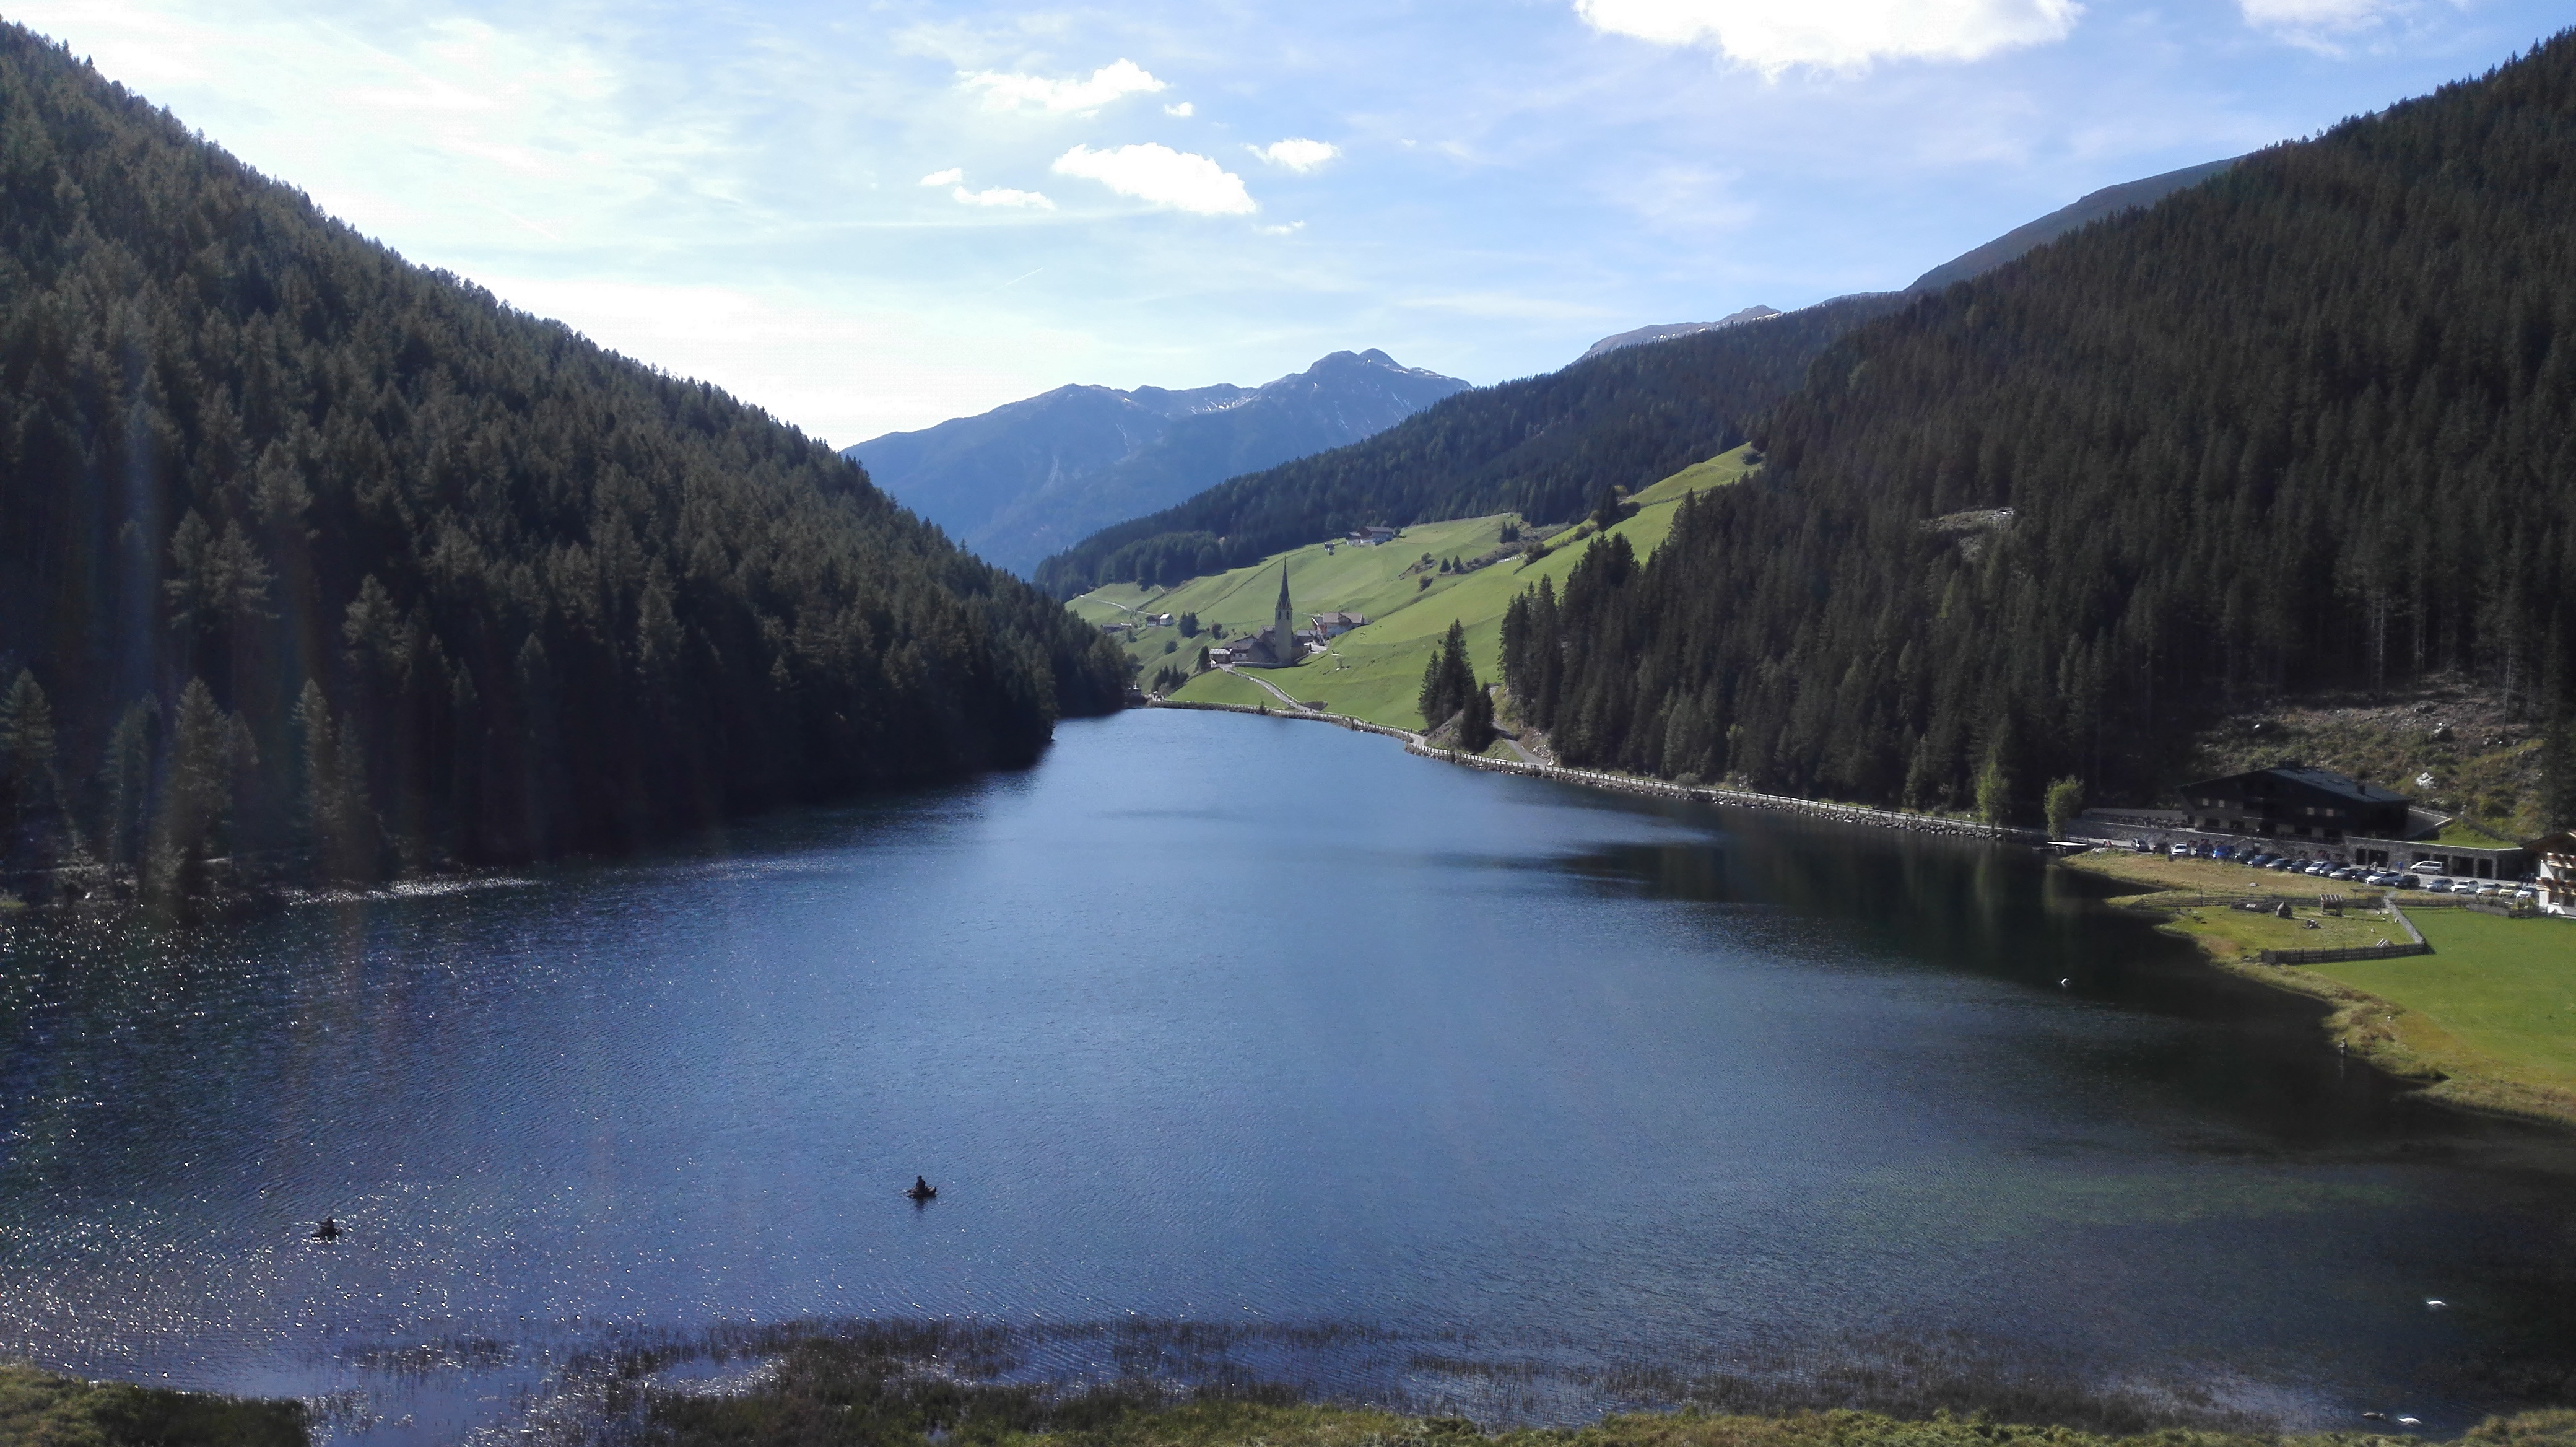
\includegraphics[scale=0.05]{img/Durnholz.jpg}%
 		\caption{Lake Durnholz where the run takes place.}\label{fig:durnholz}%
 	\end{center}%
\end{figure}
\begin{figure}[ht]%
 	\begin{center}%
 		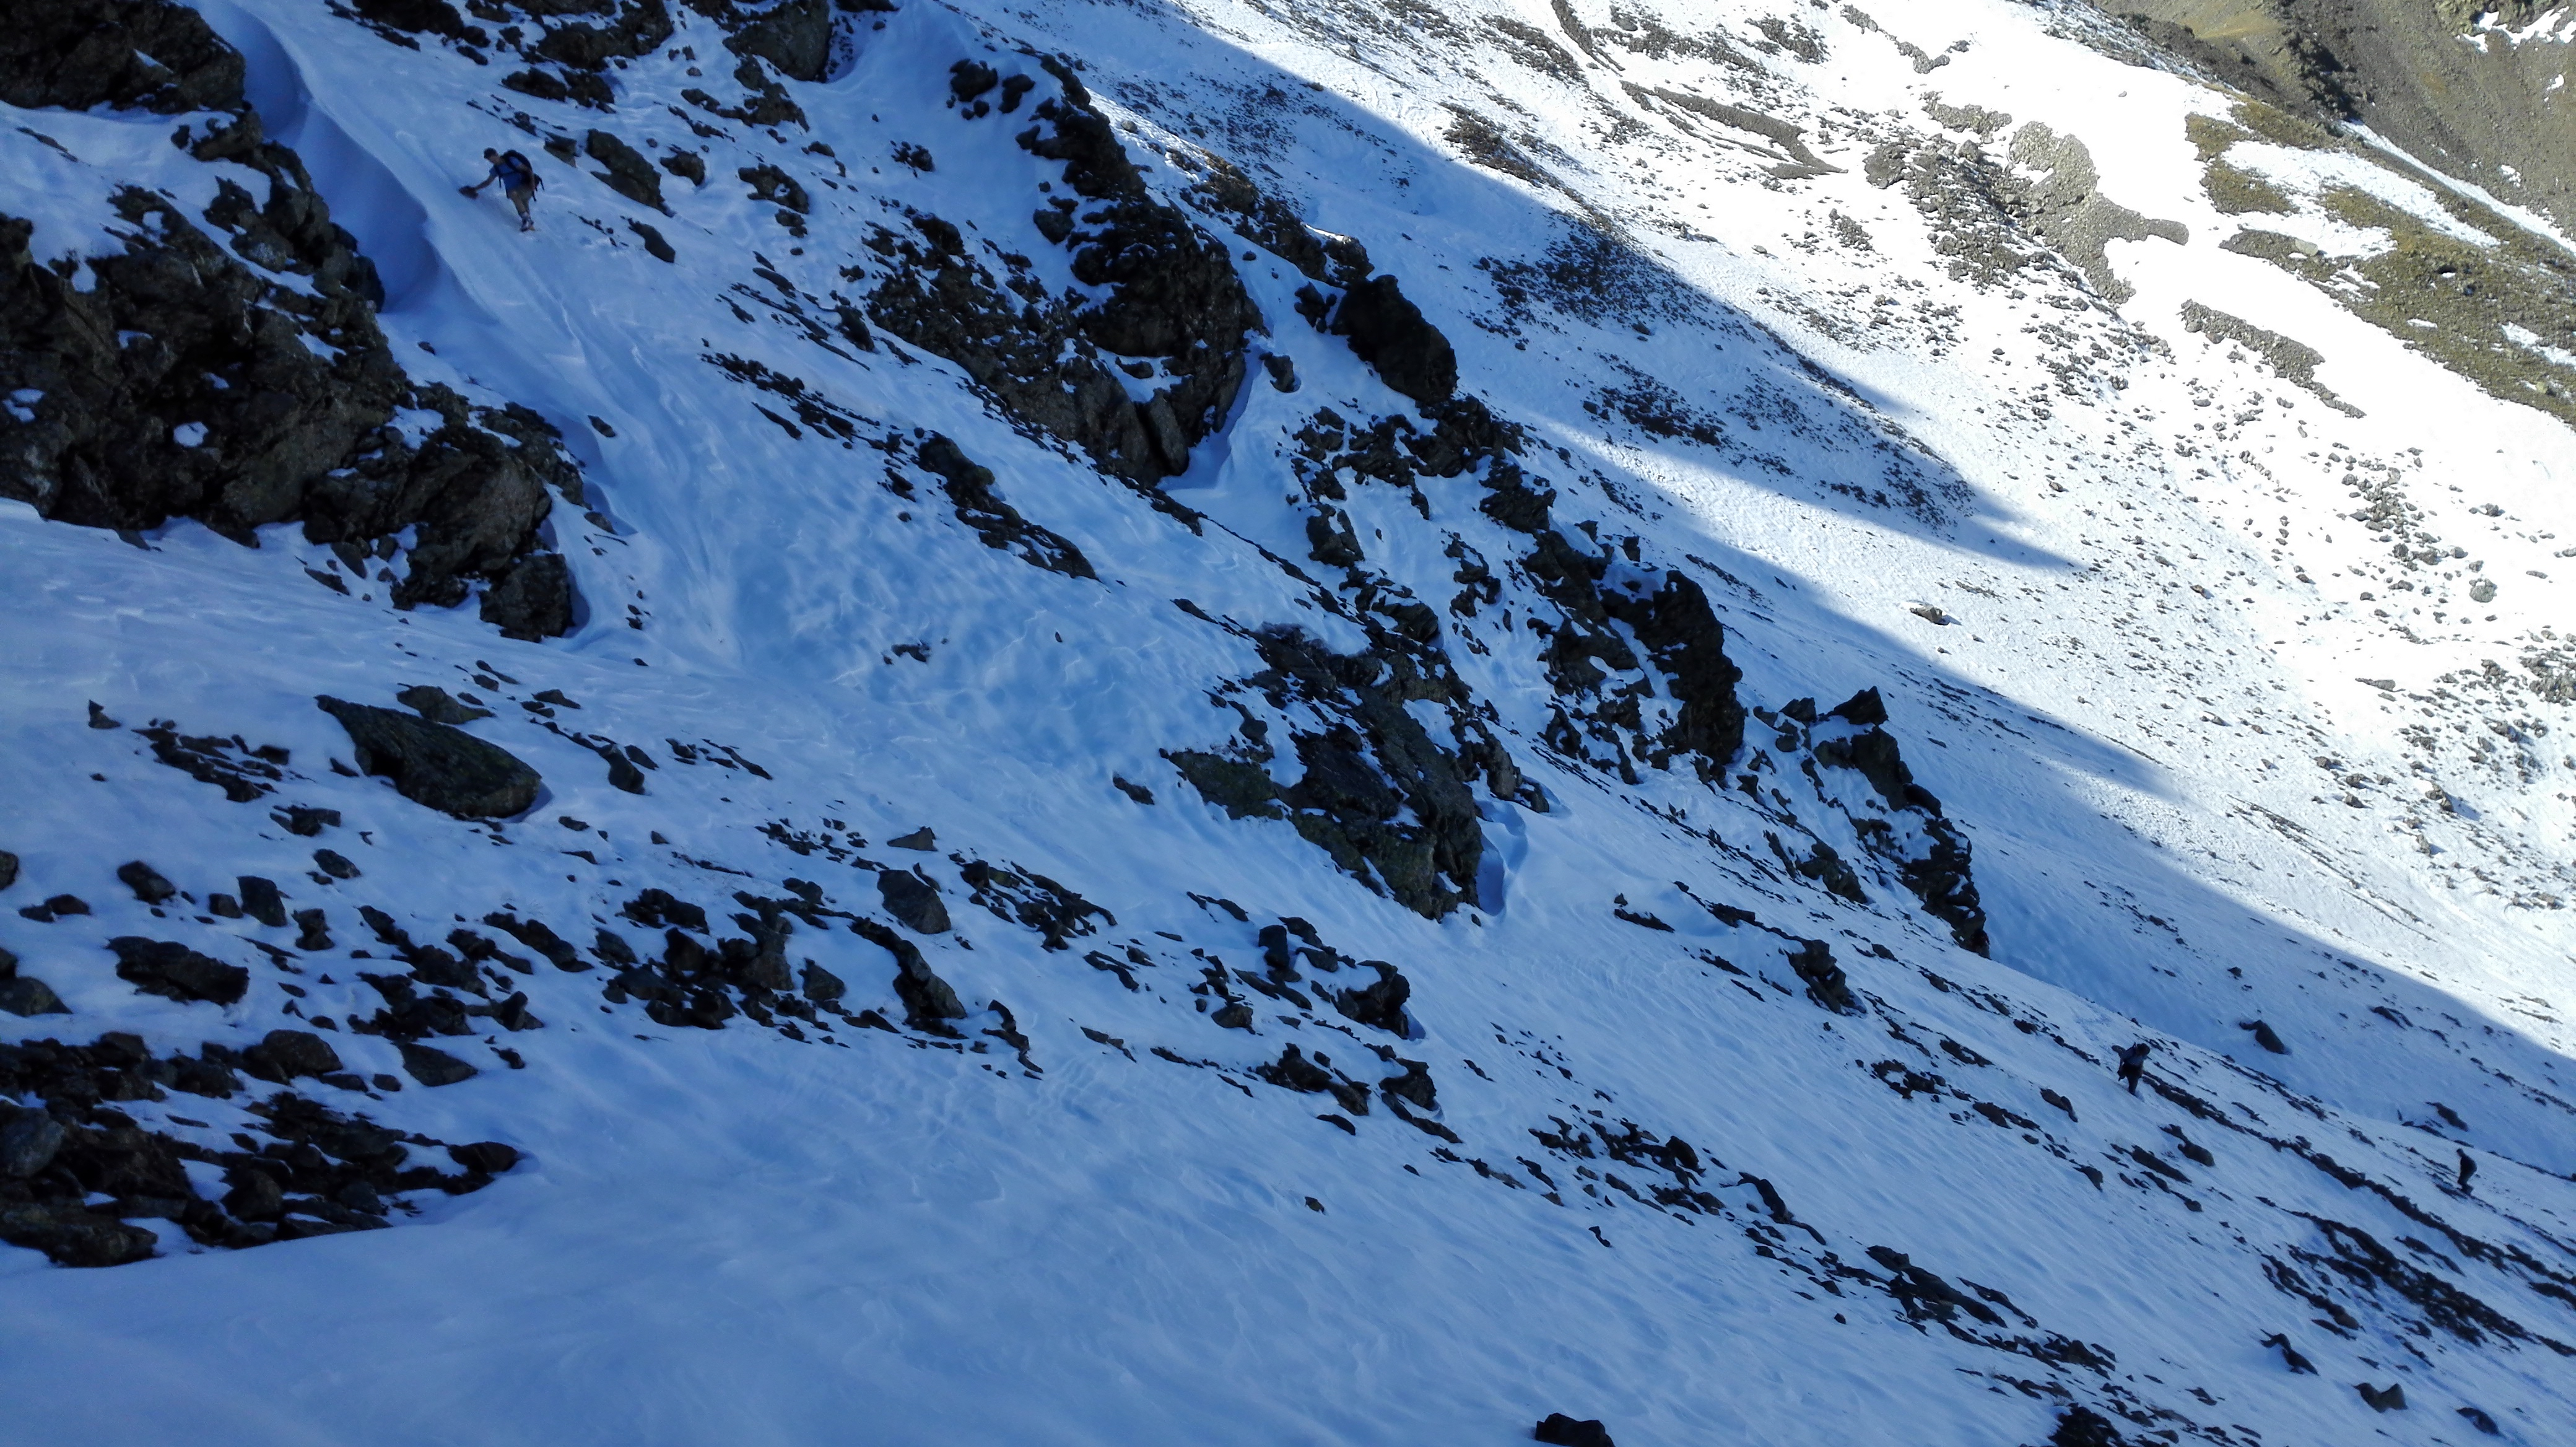
\includegraphics[scale=0.05]{img/Snow.jpg}%
 		\caption{It can become snowy as well during hikes.}\label{fig:Snow}%
 	\end{center}%
\end{figure}